%%% Local Variables:
%%% mode: latex
%%% TeX-master: t
%%% End:

%\documentclass[bachelor]{thuthesis}
%\documentclass[master]{thuthesis}
\documentclass[doctor]{thuthesis}
% \documentclass[%
%   bachelor|master|doctor|postdoctor, % mandatory option
%   secret,
%   openany|openright,
%   arialtoc,arialtitle]{thuthesis}

% 所有其它可能用到的包都统一放到这里了,可以根据自己的实际添加或者删除。
\usepackage{thutils}

% 你可以在这里修改配置文件中的定义,导言区可以使用中文。
% \def\myname{薛瑞尼}

\begin{document}

% 定义所有的eps文件在 figures 子目录下
\graphicspath{{figures/}}


%%% 封面部分
\frontmatter
%%% Local Variables:
%%% mode: latex
%%% TeX-master: t
%%% End:
\secretlevel{公开}

\ctitle{持久性内存系统中\\高效的数据一致性机制研究}
% 根据自己的情况选,不用这样复杂
\makeatletter
\ifthu@bachelor\relax\else
  \ifthu@doctor
    \cdegree{工学博士}
  \else
    \ifthu@master
      \cdegree{工学硕士}
    \fi
  \fi
\fi
\makeatother


\cdepartment[计算机]{计算机科学与技术系}
\cmajor{计算机科学与技术}
\cauthor{任晶磊}
\csupervisor{郑纬民教授}
% 如果没有副指导老师或者联合指导老师,把下面两行相应的删除即可。
%\cassosupervisor{教授}
%\ccosupervisor{教授}
% 日期自动生成,如果你要自己写就直接改这个cdate。
% 硕博也可以启用如下三行,替换其中的\the\year和\the\month为阿拉伯数字。
\CTEXdigits{\zhyear}{2015}
\CTEXnumber{\zhmonth}{12}
\cdate{\zhyear{}年\zhmonth{}月}

% 博士后部分
% \cfirstdiscipline{计算机科学与技术}
% \cseconddiscipline{系统结构}
% \postdoctordate{2009年7月——2011年7月}

\etitle{Efficient Mechanisms for\\Supporting Crash Consistency in\\Persistent Memory Systems}
% 这块比较复杂,需要分情况讨论:
% 1. 学术型硕士
%    \edegree:必须为Master of Arts或Master of Science(注意大小写)
%              “哲学、文学、历史学、法学、教育学、艺术学门类,公共管理学科
%               填写Master of Arts,其它填写Master of Science”
%    \emajor:“获得一级学科授权的学科填写一级学科名称,其它填写二级学科名称”
% 2. 专业型硕士
%    \edegree:“填写专业学位英文名称全称”
%    \emajor:“工程硕士填写工程领域,其它专业学位不填写此项”
% 3. 学术型博士
%    \edegree:Doctor of Philosophy(注意大小写)
%    \emajor:“获得一级学科授权的学科填写一级学科名称,其它填写二级学科名称”
% 4. 专业型博士
%    \edegree:“填写专业学位英文名称全称”
%    \emajor:不填写此项
\edegree{Doctor of Philosophy}
\emajor{Computer Science and Technology}
\eauthor{Jinglei Ren}
\esupervisor{Professor Weimin Zheng}
%\eassosupervisor{Professor Yongwei Wu}
\edate{December, 2015}

% 定义中英文摘要和关键字
\begin{cabstract}

新型非易失性内存介质,诸如闪存(flash)、相变内存(phase-change memory,PCM)、可变电阻式内存(ReRAM)等,可提供传统硬盘等外部存储器的数据持久化能力,和日益接近动态随机访问内存(DRAM)等内部存储器的存取性能。非易失性内存介质及其软硬件系统共同构成\emph{持久性内存}(persistent memory),可以融合传统易失性内部存储和非易失性外部存储的优良特性,提升上层应用软件和系统整体的性能和效能。

持久性内存系统使得内存数据在系统故障发生后依然得以保留。该特性在减少传统持久化机制带来的性能损耗方面作用显著,但于此同时,也使得\emph{故障时数据一致性}(crash consistency)问题尤为突出。为保证故障时数据一致性,往往需要对上层应用程序访问内存的接口加以限制。数据一致性机制及其应用程序接口方式,在持久性内存系统性能、易用性及两者间的权衡等方面扮演者至关重要的角色。

%近年提出的持久性内存系统设计通常选用基于事务(transaction)的接口,例如事务性内存等。此类解决方案虽然利用了事务接口在原子性、一致性、隔离性和持久性等方面的良好定义,但与此同时限制了持久性内存的应用范围,面临可扩展性方面的挑战,并给应用开发人员带来很大的编程负担。

%本论文研究了在持久性内存系统中提供\emph{应用透明}的访问接口的问题,以达到传统应用程序不需要更改即可利用新型持久性内存的目的。对于按块访问的非易失性内存介质(如闪存),我们基于移动系统的独特应用环境,将传统动态内存和非易失性内存整体视作一层持久性内存系统,改进现有文件系统设计,不需要手机应用实现的更改,即可以获得响应度和能耗的显著改进。对于按字节访问的非易失性内存介质(如PCM),我们完全以传统处理器内存访问指令作为接口,避免现有面向持久性内存的程序对易失性数据和非易失性数据进行划分的强制要求,内含新的双模式检查点生成技术(dual-scheme checkpointing),消除了软件编程的负担和性能瓶颈,并可应用于不作修改的遗留代码。该设计需要独特的故障时数据一致性保证机制,为此我们设计了新的数据一致性协议,并给出了其正确性的形式化证明。

本论文研究了持久性内存系统在文件系统、事务性内存和软件透明三种主要数据存取接口方式下,如何设计和实现高效的故障时数据一致性保证机制。主要创新点和研究成果包括:

\begin{itemize}
\item \emph{文件系统接口下的多版本缓存事务技术。}将原子性事务(atomic transaction)机制引入操作系统页缓存,解决由动态内存和非易失性内存构成的持久性内存系统的故障时数据一致性问题。将该技术应用于移动系统环境,在新的持久性内存系统假设下,改进现有手机文件系统设计,提出优化手机能耗和应用响应的新指标和三组新策略算法。
\item \emph{事务性内存接口下的小缓冲区组技术。}根据NVM Express接口和固态硬盘的新特性,为事务性内存设计了高效的一致性的持久化机制,构成持久性内存的一种新的实现方式。该机制包含小缓冲器组(small buffer array)的设计,在保证故障时数据一致性的同时,显著降低组提交(group commit)中提交者相互等待的时间,兼得理想的吞吐量和延迟。
\item \emph{软件透明接口下的双模式检查点生成技术。}提出支持软件透明的故障时数据一致性的混合持久性内存设计,通过双模式检查点生成技术高效地生成一致的可恢复的检查点。该技术同时在缓存块粒度和页粒度上产生检查点,可使软件执行与产生检查点的延迟重合,大幅减少停滞时间,同时实现可行的硬件空间占用。
\item \emph{软件透明的数据一致性协议及其形式化证明。}双模式检查点生成技术,对数据一致性保证提出了新的挑战。多个数据版本的隔离和维护,在程序执行和生成检查点过程重合的情况下变得尤为复杂;与此同时,硬件实现需要简单的逻辑设计。为此提出并利用状态机表达了故障时数据一致性协议;对代码级实现进行了符号抽象,利用不变式和数学归纳法对故障时数据一致性协议的正确性进行了形式化证明。
\end{itemize}

\end{cabstract}

\ckeywords{内存, 非易失性, 持久化, 事务性内存, 检查点}

\begin{eabstract}

Non-volatile memories (NVMs), such as flash, phase-change memory (PCM) and ReRAM, feature both the persistence property of external storage and the high performance of internal memory. They promise an emerging tier in the memory and storage stack.

Non-volatile memory systems ensure durability of memory data on system failures such as power outages and system crashes. This distinctive feature of NVM systems can reduce the overhead of traditional data persistence mechanisms, but introduces the critical challenge of supporting crash consistency of memory data. In order to guarantee such consistency, programs are typically limited in accessing memory data by a certain form of access interfaces. The interface choice and its corresponding consistency mechanism determine the tradeoff between programming ease and system performance.

This dissertation researches efficient consistency mechanisms and/or system performance optimizations for NVM systems, under three main forms of interfaces, file system, transactional memory, and the software-transparent. The main contributions of this dissertation include the following.

\begin{itemize}
\item For file systems, we introduce atomic transactions to the page cache of operating systems to ensure that memory data is flushed to persistent storage in a consistent manner. This technique is applied to smartphones whose DRAM can be assumed as a NVM system, in order to optimize energy efficiency and app responsiveness. We design app-adaptive policies and algorithms to quantatively trade off between data staleness and energy efficiency/app responsiveness.

\item For transactional memories, we propose a new buffering and group commit design, the small buffer array, according to the characteristics of (potentially NVRAM-enhanced) NVM Express-attached flash cards. It largely reduces the waiting latency in group commit, while saturating the bandwidth of the flash cards. Moreover, we employ snapshot isolation to hide write latency from the critical path of read-only transactions, which brings significant performance improvement to real-time analytical workloads.

\item With software-transparent interfaces, programs can safely access memory data using regular load/store instructions. Programmers do not need bother partitioning transient and persistent data or writing transactional code, and enjoy better portability than using particular transaction libraries. To enable this approach, we propose a highly efficient consistent cooperative checkpointing mechanism which synchronously checkpoints memory data at different granularities.

\end{itemize}

\end{eabstract}

\ekeywords{memory, persistence, non-volatile, transactional memory,
checkpointing}


% 设置 PDF 文档的作者、主题等属性
\makeatletter
\thu@setup@pdfinfo
\makeatother
% 如果使用授权说明扫描页,将可选参数中指定为扫描得到的 PDF 文件名,例如:
%\makecover[scan-auth.pdf]
\makecover

% 目录
\tableofcontents

% 符号对照表
\begin{denotation}
\item[ACID] 原子性(atomicity)、一致性(consistency)、隔离性(isolation)和持久性(durability)
\item[DRAM] 动态随机访问内存(dynamic random access memory)
\item[I/O] 输入与输出
\item[PCM] 相变内存(phase-change memory)
\item[$s$] 表征数据滞后量(staleness)的值
\item[$e$] 表征能量节约的量与数据滞后量的比值
\end{denotation}



%%% 正文部分
\mainmatter
\chapter{绪论}
\label{chap:intro}

传统计算机存储包括内存和外存两层架构。内存采用高性能但具有易失性的随机访问存储器(dynamic random access memory,DRAM),而外存采用非易失性的但性能较弱的块设备,如机械硬盘。
相应地,操作系统设计了虚拟内存和I/O系统\cite{Galvin:2013:OSC:2531466,Tanenbaum:2014:MOS:2655363}来完成对两种形态数据的协调和管理,不可避免地带来诸多性能和管理开销\cite{Lang:1977:DBP:320576.320585,Yu:2014:OBI:2642648.2619092}。

近年来,科研人员开发出一类非易失性内存,融合了传统内存的高性能和随机访问特性,以及传统外存的持久化和非易失特性。典型的非易失性内存介质包括闪存\cite{705361,542301}、自旋扭矩转换内存(spin-torque transfer RAM,STT-RAM)\cite{4443191,6557176}、相变内存(phase-change memory,PCM)\cite{Loke22062012,6176872,Raoux:2008:PRA,10.1109/MM.2010.24}以及电阻式内存(ReRAM)\cite{5607274}等。

非易失性内存有望改变传统的双层存储架构,构成内外存统一的\emph{单层}存储系统。我们将围绕非易失性存储介质的软硬件系统称为\textbf{持久性内存系统}。它使得内存数据在系统故障发生后依然得以保留。单层的持久性内存系统可以减少数据在内存和外存之间的传输、在内存数据结构和外存数据结构之间的转换、相关的系统调用等开销\cite{meza2013case}。

新的持久性内存系统在展现诱人前景的同时,亦面临着诸多技术挑战,诸如非易失性内存硬件的耐久性、纠错等(第\ref{intro:nvm-review}节)。这些问题在硬件层面可以得到较好的解决。然而,\textbf{故障时数据一致性}(crash consistency)问题(第\ref{intro:crash-consistency}节)由于同时涉及软硬件系统且对性能优化的要求高而变得尤为棘手。数据一致性是应用程序对存储系统不可或缺的最基本要求之一,所以该问题成为持久性内存在实际中应用的一个重大障碍\cite{Onur:2014:RPO}。基于此,本论文聚焦于为持久性内存系统支持故障时数据一致性研究高效的软硬件机制和策略。

在数据一致性机制的设计中,面向应用的接口扮演着重要的角色。接口方式和语义决定了持久性内存系统的易用性,也决定了性能和效能优化的空间。在整个软硬件系统栈中,文件系统、事务性内存和对软件透明的硬件接口代表了三类典型的接口方式。\textbf{本论文系统研究了采用文件系统、事务性内存和软件透明三种主要数据存取接口方式下,如何为持久性内存系统设计和实现高效的故障时数据一致性保证机制的问题。}本文主要研究内容和成果包括:

\begin{itemize}
\item 文件系统接口下持久性内存系统的故障时数据一致性机制。设计了\textbf{多版本缓存事务技术},通过将原子性事务(atomic transaction)机制引入操作系统页缓存,解决由动态内存和非易失性内存构成的持久性内
存系统的故障时数据一致性问题。将该技术应用于移动系统环境,在新的持久性内存系统假设下,改进现有手机文件系统设计,提出优化系统能耗和应用响应的新指标和新策略算法。
\item 事务性内存接口下持久性内存系统的故障时数据一致性机制。根据NVM Express\cite{nvme}接口和固态硬盘的新特性,为事务性内存设计了一种高效的具有一致性保证的持久化机制,为持久性内
存提供了一种新的实现方式。该机制包含\textbf{小缓冲区组}的新技术(small buffer array)。该技术在保证故障时数据一致性的同时,显著降低组提交(group commit)中提交者相互等待的时间,兼得理想的吞吐量和延迟。
\item 对软件透明的持久性内存系统故障时数据一致性机制。提出支持软件透明的故障时数据
一致性的混合持久性内存设计,和\textbf{双模式检查点生成技术}。通过双模式检查点生成技术高效地生成一致的可恢复的检查点。该技术同时在缓存块粒度和页粒度上产生检查点,可使软件执行与产生检查点的延迟重合,大幅减少停滞时间,而仅占用较小的硬件空间。
\item 对软件透明的故障时数据一致性协议及其形式化证明。双模式检查点生成技术,对数据一致性保证提出了新的挑战。多个数据版本的隔离和维护,在程序执行和生成检查点过程重合的情况下变得尤为复杂;与此同时,硬件实现需要简单的逻辑设计。为此我们提出并利用状态机模型表达了故障时数据一致性协议。同时,我们还对代码级实现进行了符号抽象,利用不变式和数学归纳法对故障时数据一致性协议的正确性进行了形式化证明。
\end{itemize}

\section{非易失性内存相关技术回顾}
\label{intro:nvm-review}

部分非易失性内存介质,如PCM,面临耐久性问题。磨损均衡(wear leveling)和比特映射(bit mapping)是解决该问题,扩展非易失性内存介质耐久性的典型技术。在磨损均衡技术中,行移动(row shifting)可以避免一个行内各存储单元上热点区域对存储介质的损害,而段交换(segment swapping)\cite{Qureshi:2009:SHP:1555754.1555760}可以平衡对页的使用\cite{Zhou:2009:DEE:1555754.1555759}。起始间隔(Start-gap)技术\cite{Qureshi:2009:SHP:1555754.1555760}维护从逻辑内存地址到物理内存地址的代数映射关系,而不依靠追踪内存写得到的统计结果。

另一方面,科研人员希望减少冗余的比特粒度的写入。传统存储系统在页或块粒度上向持久性介质写入数据,而这些页或块的内部有相当的比例并没有被更改。对于PCM等非易失性内存,最佳的方式是未修改的比特位可以不写入内存介质。文献\cite{Zhou:2009:DEE:1555754.1555759}利用PCM读性能显著优于写性能的特性,在每次写之前读出原有数据来定位未修改的比特位。Flip-N-Write\cite{5375405}技术给每个PCM上的字附加一位翻转标记,来表明物理的0或1与逻辑的0或1的对应关系。当这个字被修改时,通过计算最小的比特重置的数量来设置该翻转标记位,从而减少比特级的写入量,获得性能、能耗和耐久性等的提升。

错误修复对非易失性内存有着特别的意义,因为与易失性内存不同,非易失性内存保存的数据具有持久性,一旦发生错误代价更为高昂。考虑到PCM相对DRAM而言耐久性弱,错误恢复技术多选择内置在硬件中。动态复制内存技术\cite{Ipek:2010:DRM:1736020.1736023}保存一个页的两个副本,而Zombie\cite{Azevedo:2013:ZME:2485922.2485961}则针对单层存储单元(single-level cell,SLC)和多层存储单元(multi-level cell,MLC)的结构,提出和扩展了多种内存错误修复技术。

\section{持久性内存系统的数据一致性问题}
\label{intro:crash-consistency}

故障时数据一致性是持久性内存系统面临的最为棘手的问题之一\cite{Onur:2014:RPO}。故障时数据一致性的定义是,系统发生故障并恢复后,内存数据呈现为历史上时间点$t$时的快照,即所有$t$之前的内存写按其接收顺序体现在数据存储中而所有$t$之后的内存写都不保存。

数据不一致会给应用程序带来很多严重错误。例如悬空指针(dangling pointer)问题\cite{Volos:2011:MLP:1950365.1950379,Coburn:2011:NMP:1950365.1950380}。假设一个应用在持久性内存中写入了一组特定的数据,并使用一个指针引用这些数据。系统故障恢复后,如果先写入的数据丢失了,而后写入的指针被保留(违背上述时间点$t$的一致性定义),那么程序后续一旦使用该悬空指针就可能引发严重的运行时异常或错误。再比如经典的原子更新问题。假设客户要求从银行账户A中减除部分数额的资金加到银行账户B上。如果标志操作原子性完成的写先于对账户A的写\emph{或}对账户B的写发生,那么一旦系统中途发生故障,回滚的状态违背一致性定义,就可能出现账户A钱少了而账户B未加钱(或者相反)的状况。这显然无法满足程序语义上的要求,可能对各方系统用户造成重大损失。

\section{本文内容及结构}

为了解决持久性内存系统中数据一致性保证的问题,我们从文件系统作为访问接口、事务性内存作为访问接口和对软件透明的三个角度进行了研究,分别对应于第\ref{chap:vct}章、第\ref{chap:sba}章和第\ref{chap:thynvm}章的内容。这三个角度涵盖了持久性内存系统最主要的接口方式。此外,软件透明的一致性协议具有一定复杂度且是相对独立的重要贡献,其定义及证明放置在第\ref{chap:protocol}章。第\ref{chap:conclusion}章总结了本文工作并对未来方向寄予了展望。


\chapter{多版本缓冲事务技术及文件系统效能优化}
\label{chap:vct}

\section{文件系统及效能优化}

\subsection{现有文件系统设计和页缓存}

\subsection{文件系统对应用效能的影响}

\subsection{数据一致性和滞后性}

\section{以内存为中心的文件系统}

\subsection{设计原则}

\subsection{系统架构}

\begin{figure}
  \centering
  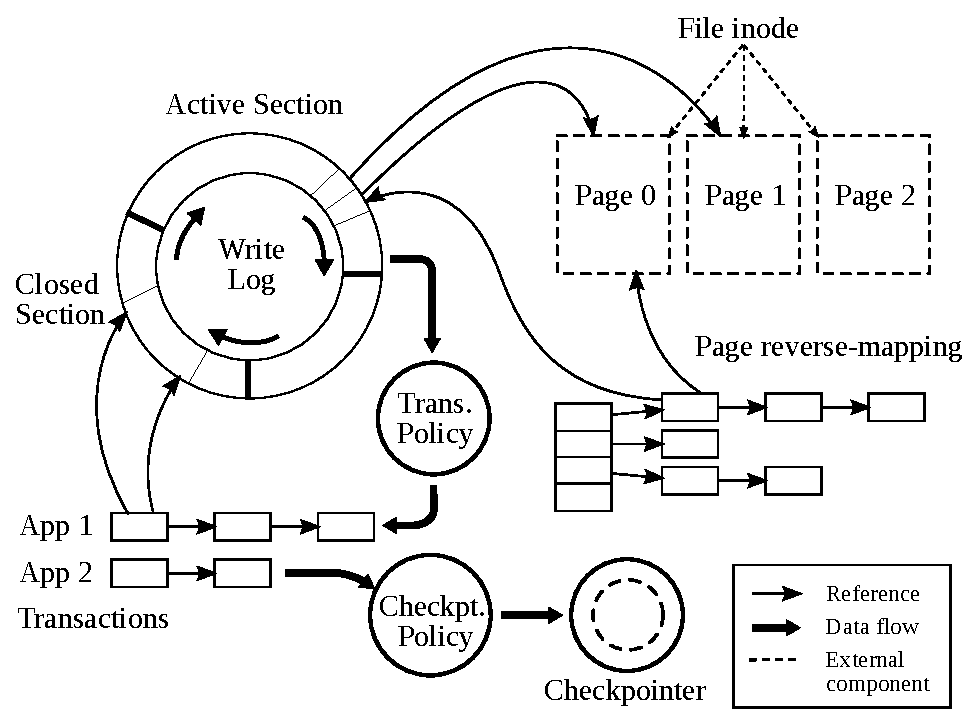
\includegraphics[width=0.8\columnwidth]{arch}
  \caption{MobiFS系统架构图}
  \label{fig:arch}
\end{figure}

MobiFS主要由五个模块构成:(1)页缓存,负责在内存中存储文件数据;(2)写日志,负责维护写操作的历史,由按序排列的许多记录项构成;(3)事务,写日志中的若干记录项归并为一组,它们的一致性不受覆写和重排序等优化的影响;(4)检查点生成器(checkpointer),负责调用底层闪存存储组件以原子性方式完成事务的持久化;(5)策略引擎,负责依据优化算法划分事务的边界,监听用户交互行为,并决定生成检查点的事务和时机。图~\ref{fig:arch} 描绘了MobiFS的系统架构。

MobiFS的设计充分考虑了与现有操作系统(Linux)的兼容和组件重用。它与操作系统共享现有的页缓存结构。对于页缓存的每个写操作,都会记入写日志,通常体现为在当前事务中(写日志的末尾)追加一个记录项,除非当前事务已经包含目标页地址的记录项。为此,我们需要维护一组从页地址到写日志项的逆向映射,以判断目标页地址是否已经存在于事务中。基于写日志和逆向映射,MobiFS建立起原子性事务机制。每个事务定义了可以进行覆写和重排序等优化的一个特定范围。最终,策略引擎指导检查点生成器保存事务到闪存,同时不影响用户交互。策略引擎根据每个手机应用甚至是用户的行为及其统计指标,做出动态的智能的判断。

在一个典型的配置中,不同手机应用会拥有自己独立的写日志和事务,但它们共享逆向映射、策略引擎和检查点生成器等组件。

\section{多版本缓冲事务技术}

\subsection{写日志}

写日志是应用所有写操作按时间排列的历史记录。写日志包含两个段:活跃段(active section)处在写日志的末尾,新的记录项会被插入活跃段;闭合段(closed section)则包含准备生成检查点的记录项。 
 
在Android平台上,一份写日志的范围涵盖一个手机应用访问的所有目录。手机应用可能使用数据库SQLite保存数据,而SQLite是一个嵌入式数据库,它与每个应用捆绑的相关文件也需要托管给MobiFS,包含在应用的写日志范围内。
 
我们之所以能够面向特定应用进行写优化,一个重要原因在于手机应用的数据路径是静态的和相互隔离的,从而避免了应用间的一致性问题。当然,的确存在多个应用共享文件数据的情况,例如文件浏览器和相册应用可能同时管理照片存放的目录。这种情况下,相关应用需要在程序逻辑层面进行处理。即便不使用MobiFS,在现有Android的文件系统上,应用同样需要处理这类情况(例如,用户通过文件浏览器手动删除了相册中原本可见的照片)。 

\subsection{事务和版本}

在写日志中,可能同时存在逻辑上同一个缓冲页的多个物理版本。多版本缓冲事务用来管理这种关系。一个多版本缓冲事务在其生命周期内经历三个状态:(1)当处于打开状态时,一个事务接收新的记录项,而这些记录项构成写日志中的活跃段。(2)当进入闭合状态时,该事务的所有记录项不再可以更改,转入写日志的闭合段。从打开状态到闭合状态的转换是单向的,不可逆的。(3)当进入提交状态时,该事务所有记录项对应的物理缓存页被检查点生成器原子性地刷出到闪存。成功提交之后,该事务及其记录项即从写日志中消除。 
 
覆写和重排序等优化手段只允许用于单个多版本缓冲事务内部。由于检查点生成器可保证一个事务整体的持久化和原子性,这些优化不会导致闪存数据的任何不一致状态。 
 
当一个写操作到达时,MobiFS需要处理三种情况:(1)如果要写入的目标页不存在于逆向映射中,那么意味着写操作将进入一个未被写日志涵盖的页。MobiFS会在写日志中追加一个记录项,建立到缓存页的映射,并建立逆向映射。(2)如果逆向映射已经存在且指向一个写日志闭合段中的记录项,那么意味着写操作想要写入一个被保护的只读的事务。为此MobiFS对目标页执行写时拷贝(copy-on-write),并为新的页副本添加写日志记录项及映射/逆向映射。(3)如果逆向映射存在且指向一个写日志活跃段中的记录项(即打开的事务),那么意味着目标页不在被保护的闭合事务中,写操作可以直接更改目标页。

\subsection{故障恢复}

\subsection{检查点生成}

\section{效能优化策略和算法}

\subsection{概述}

\subsection{事务划分算法}

\subsection{行为间隔预测}

\subsection{事务调度}

\section{系统实现和效能评测}

\subsection{系统实现}

\subsection{评测方法}

\subsection{内存占用评测}

\subsection{应用和用户感知评测}

\subsection{应用响应度评测}

\subsection{能耗评测}

\section{本章小结}




%%% 其它部分
\backmatter

% 本科生要这几个索引,研究生不要。选择性留下。
\makeatletter
\ifthu@bachelor
  % 插图索引
  \listoffigures
  % 表格索引
  \listoftables
  % 公式索引
  %\listofequations
\fi
\makeatother


% 参考文献
% 注意至少需要引用一篇参考文献,否则下面两行可能引起编译错误。
% 如果不需要参考文献,请将下面两行删除或注释掉。
\bibliographystyle{thubib}
\bibliography{ref/refs}


% 致谢
%%% Local Variables:
%%% mode: latex
%%% TeX-master: "../main"
%%% End:

% 如果使用声明扫描页,将可选参数指定为扫描后的 PDF 文件名,例如:
%\begin{ack}[scan-statement.pdf]
\begin{ack}

衷心感谢导师郑纬民教授和武永卫教授。他们在学术上悉心指导,在生活上关心照顾,为学生的发展构建了广阔的平台。忘不了和老师们的一次次讨论,忘不了老师们的谆谆教诲,也忘不了武老师在我的婚礼上作为主婚人的温馨致辞。

我还要感谢以往论文的其他合作者和指导者,他们的智慧亦融合在我的毕业论文中。微软亚洲研究院的Thomas Moscibroda和Mike Liang研究员为MobiFS项目的策略设计给予了宝贵建议。卡內基·梅隆大学(Carnegie Mellon University)的Onur Mutlu教授帮助我挖掘想法中价值,和时任惠普实验室(HP Labs)研究员的Jishen Zhao博士、时任英特尔研实验室(Intel Labs)研究员的Samira Khan博士一起反复修改我的论文。斯坦福大学(Stanford University)的David Cheriton教授和Heiner Litz博士多次斧正我的想法,他们组的工作为我的论文提供了很好的基础。我合作的论文中,当时威斯康星大学麦迪逊分校(University of Wisconsin–Madison)的Shan Lu教授给予的帮助和指导,在此一并感谢;原SanDisk副总裁John Butsh博士、Facebook工程师Justin Meza博士对论文工作的判断和帮助也令我受益匪浅。此外,特别感谢清华实验室的陈康老师、蒋进磊老师、黄小猛老师、杨广文老师等多年来寄予的指导和照顾;师兄弟刘立坤、张扬、祝美祺、章明星、王博、郭维超、赵勋、牟帅、王秋平、叶丰、苏茂萌、高品等同学,不断和我分享着他们的创见、努力和一起玩乐的美好时光。

感谢我的妻子闫睿颖女士,她无私无畏的支持和先于我工作所给予的经济援助,帮我度过了无数难关。儿子任念初的到来,赐予我生命的灵感和前行的动力。更要感谢我的父母任东兴、任焕茹,我的岳父母闫子政、张世平,他们构筑了我多年科研工作的坚实后方,是我毕业论文能够成文的不可磨灭的功臣。

最后,感谢自然科学基金、国家863计划、国家973计划、清华大学博士生短期出国访学基金、清华大学信息科学技术学院登峰基金、斯坦福大学计算机科学系等对本人工作的资助。感谢答辩委员会专家及匿名评审专家的宝贵时间和指导。

\end{ack}


% 附录
\begin{appendix}
\input{data/appendix01}
\end{appendix}

% 个人简历
\begin{resume}

  \resumeitem{个人简历}

  1986 年 9 月 12 日出生于河北省保定市。

  2006 年 9 月考入东北师范大学软件学院软件工程专业,2010 年 7 月本科毕业并获得工学学士学位。

  2010 年 9 月免试进入清华大学计算机科学与技术系攻读硕士学位;2013 年 7 月转为提前攻读博士学位至今。

  博士在读期间,2013 年 11 月至 2014 年 5 月在卡内基梅隆大学(Carnegie Mellon University)电子与计算机工程系做访问研究;2014 年 10 月至 2015 年 8 月在斯坦福大学(Stanford University)计算机科学系做访问研究。

  \researchitem{发表的学术论文} % 发表的和录用的合在一起
% 学位论文写作指南:
% 在学期间发表的学术论文分以下三部分按顺序分别列出,每部分之间空 1
% 行,序号可连续排列
% 1. 已经刊载的学术论文(本人是第一作者,或者导师为第一作者本人是第二作者)
% 2. 尚未刊载,但已经接到正式录用函的学术论文(本人为第一作者,或者
% 导师为第一作者本人是第二作者)。
% 3. 其他学术论文。可列出除上述两种情况以外的其他学术论文,但必须是
% 已经刊载或者收到正式录用函的论文。
  \begin{publications}
  \item \textbf{Jinglei Ren}, Jishen Zhao, Samira Khan, Jongmoo Choi, Yongwei Wu, and Onur Mutlu.
ThyNVM: Enabling Software-Transparent Crash Consistency in Persistent Memory Systems.
In Proceedings of the 48th Annual IEEE/ACM International Symposium on Microarchitecture (MICRO), pp. 672 - 685, Dec. 2015.(CCF 推荐 A 类会议)
  \item \textbf{Jinglei Ren}, Chieh-Jan Mike Liang, Yongwei Wu, and Thomas Moscibroda.
Memory-Centric Data Storage for Mobile Systems.
In Proceedings of the 2015 USENIX Annual Technical Conference (USENIX ATC), pp. 599 - 611, Jul. 2015.(CCF 推荐 B 类会议)
  \item \textbf{Jinglei Ren}, Yongwei Wu, Meiqi Zhu, and Weimin Zheng.
Quatrain: Accelerating Data Aggregation Between Multiple Layers.
IEEE Transactions on Computers (TC), Vol. 63, No. 5, pp. 1207 - 1219, May 2014. (CCF 推荐 A 类期刊,SCI 检索)
  \item Mingxing Zhang, Yongwei Wu, Shan Lu, Shanxiang Qi, \textbf{Jinglei Ren}, and Weimin Zheng.
AI: A Lightweight System for Tolerating Concurrency Bugs.
In Proceedings of the 22nd ACM SIGSOFT International Symposium on the Foundations of Software Engineering (FSE), pp. 330 - 340, Nov. 2014.(CCF 推荐 A 类会议)
  \item Yongwei Wu, Weichao Guo, \textbf{Jinglei Ren}, Xun Zhao, and Weiming Zheng.
NO2: Speeding Up Parallel Processing of Massive Compute-Intensive Tasks.
IEEE Transactions on Computers (TC), Vol. 63, No. 10, pp. 2487 - 2499, Oct. 2014.(CCF 推荐 A 类期刊,SCI 检索)
  \end{publications}

  \researchitem{研究成果} % 有就写,没有就删除
  \begin{achievements}
  \item 武永卫、 郑纬民、陈康、任晶磊: 远程调用方法及系统. (中国专利申请号:201310646738.0)
  \end{achievements}
\end{resume}


\end{document}

